\subsection{Interface Mémoire}

Le module de mémoire a été conçu de manière générique à l'aide d'interfaces java. Pour cela elle se décompose en trois parties :

\begin{itemize}
\item l'interface principale de la mémoire (\texttt{Memory}), qui déclare les méthodes appelées par les autres modules (Analyse et Raisonnement), et qui est implémentée en tant que mémoire à court terme (\texttt{ActiveMemory}),

\item l'interface de la mémoire épisodique (\texttt{EpisodicMemory}) et l'interface de la mémoire sémantique (\texttt{SemanticMemory}), qui déclarent les méthodes appelées par les implémentations de l'interface \texttt{Memory}.
\end{itemize}

\begin{figure}[H]
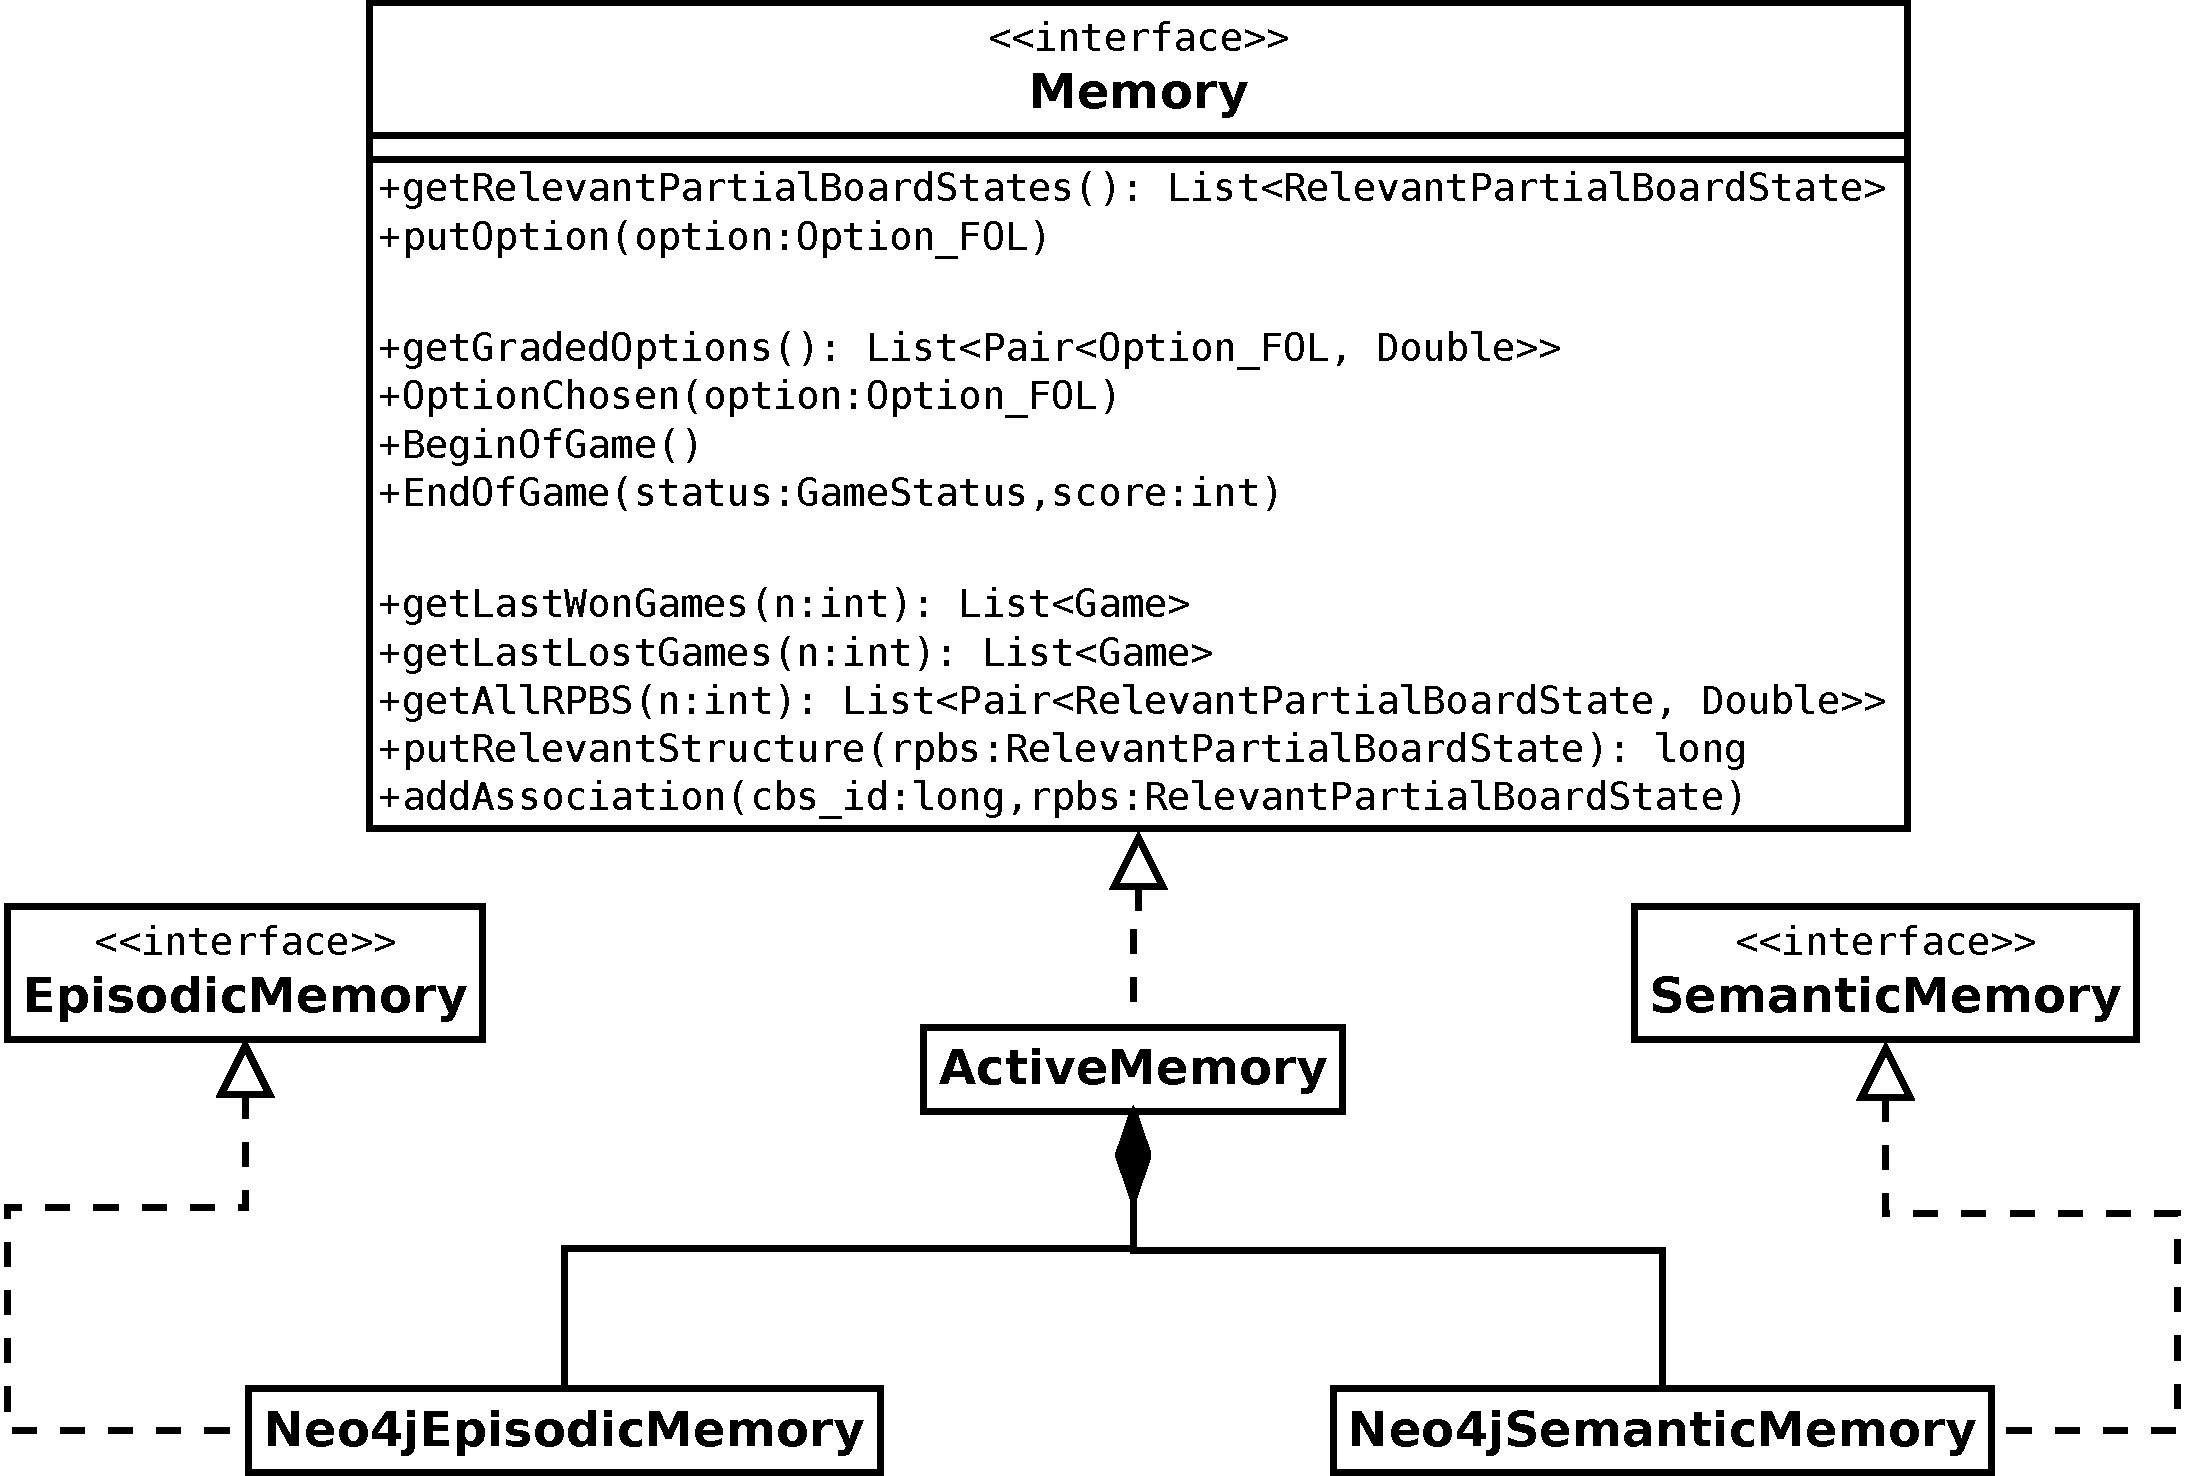
\includegraphics[width=\textwidth]{files/memoire/interface}
\caption{Diagramme de classe du module mémoire simplifié.}
\end{figure}

La mémoire assure également la persistance des données, qui se fait via un module de persistance qui est utilisé les implémentations \texttt{Neo4jEpisodicMemory} et \texttt{Neo4jSemanticMemory}. 

\subsection{Le \gls{SGBD} Neo4j}

La persistance des données est assurée par un \gls{SGBD} né de la mouvance \gls{NoSQL} : Neo4j. Il permet la gestion d'une base de données orientée graphe. Nous avons fait le choix d'utiliser un tel système pour plusieurs raisons :

\begin{itemize}
\item nous avions la volonté de \textbf{découvrir une solution \gls{NoSQL}}, que nous n'avons pas eu l'occasion d'étudier lors de notre formation,

\item Neo4j est disponible en \textbf{plusieurs versions}, notamment en version serveur, version webservice REST et version java embarquée. La mémoire ne nécessitant pas d'accès concurrents mais aussi par soucis de légèreté, c'est la version embarquée (\emph{embedded java}) qui a été utilisée,

\item ce type de \gls{SGBD} \gls{NoSQL} permet d'obtenir des \textbf{temps d'accès} plus rapides qu'avec des \gls{SGBD} relationnels traditionnels,

\item la vision graphe de la base de données est \textbf{adaptée} à la conception de notre mémoire\footnote{Notons tout de même qu'il aurait était été possible de stocker les données sous forme de tables relationnelles classiques.},

\item cette solution conserve les \textbf{propriétés \gls{ACID}} des transactions des \gls{SGBD} relationnels traditionnels,

\item la \textbf{documentation complète} et la \textbf{communauté active} permettent de s'initier très rapidement à cette nouvelle technologie,

\item Neo4j est une \textbf{solution libre} distribuée sous licence \gls{GPLv3}.
\end{itemize}

Neo4j étant un \gls{SGBD} \gls{NoSQL} orienté graphe, la base de donnée est représentée sous la forme d'un graphe orienté, composé d'un nœud \og root \fg{}. Chaque nœud et chaque arc peut posséder des attributs. Cependant, il n'est possible de typer que les arcs. Pour typer les nœuds une astuce consiste en la création d'un \og master\_node \fg{} comme le montre la figure~\ref{example_node_type}.

\begin{figure}[H]
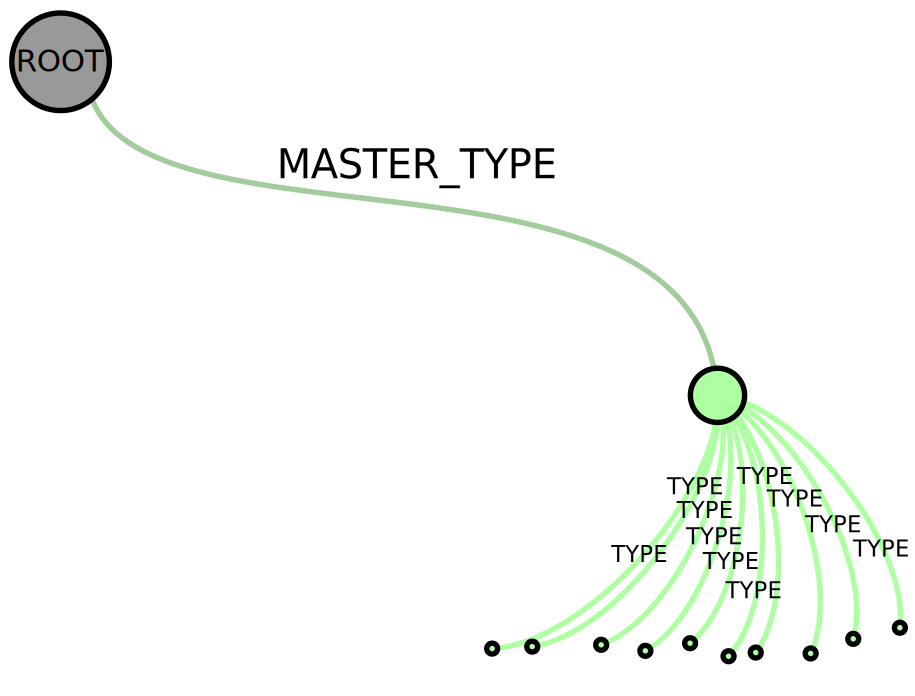
\includegraphics[width=\textwidth]{files/neo4j/example_node_type}
\caption{Exemple de typage des noeuds avec Neo4j.}
\label{example_node_type}
\end{figure}

\subsection{Éléments en mémoire}

Le module de persistance permet le stockage de la mémoire épisodique et sémantique, les deux étant liées par les relations entre les \emph{MOVE} et les \emph{OBJECTS}. Nous avons donc besoin des types suivants : 

\textbf{Types de noeud :}
\begin{itemize}
	\item \texttt{GAME} : une partie en mémoire épisodique, 
	\item \texttt{MOVE} : un coup joué en mémoire épisodique,
	\item \texttt{OBJECT} : un plateau en mémoire sémantique,
	\item \texttt{ATTRIBUTE} : une forme remarquable en mémoire sémantique.
\end{itemize}


\textbf{Types de liens :}
\begin{itemize}
	\item Relations maitres
		\begin{itemize}
			\item \texttt{MASTER\_ATTR},
			\item \texttt{MASTER\_OBJ},
			\item \texttt{MASTER\_GAME},
			\item \texttt{MASTER\_MOVE}.
		\end{itemize}
	\item Relations de type
		\begin{itemize}
			\item \texttt{ATTRIBUTE},
			\item \texttt{OBJECT},
			\item \texttt{MOVE},
			\item \texttt{GAME},
			\item \texttt{LAST\_GAME} (relation \texttt{GAME} spéciale, signifiant que cette partie est la dernière jouée).
		\end{itemize}
	\item Relations en mémoire épisodique
		\begin{itemize}
			\item \texttt{PREV\_GAME} : permet à partir d'une partie d'accéder à la précédente,
			\item \texttt{LAST\_MOVE} : permet à partir d'une partie d'accéder au dernier coup joué,
			\item \texttt{PREV\_MOVE} : permet à partir d'un coup d'accéder au précédent,
			\item \texttt{STATE\_BOARD} : permet de lier un coup à l'état de plateau correspondant.
		\end{itemize}
	\item Relations en mémoire sémantique
		\begin{itemize}
			\item \texttt{RELATED} : décrit la présence d'une forme remarquable (\texttt{ATTRIBUTE}) dans un plateau (\texttt{OBJECT}).
		\end{itemize}
	\end{itemize}
	
\subsection{Mémoire sémantique}
Comme vu dans la partie~\ref{conception_memoire_semantique} (page \pageref{conception_memoire_semantique}, la mémoire sémantique stocke une matrice de booléens ayant comme attributs (colonnes) des formes remarquables, et comme objets (lignes) des plateaux.

On peut voir sur la figure~\ref{lattice_graph} les deux \og master\_node \fg{} permettant de déclarer des nœuds d'attributs et d'objets. Ces nœuds sont en liés via des relations de type \emph{RELATED}.

\begin{figure}[H]
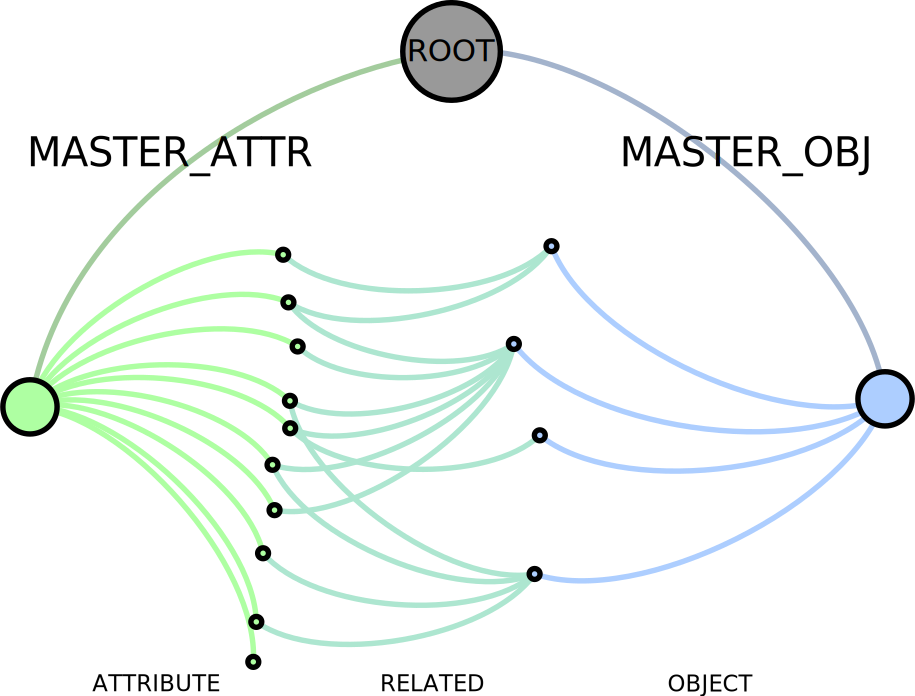
\includegraphics[width=\textwidth]{files/neo4j/lattice_graph}
\caption{Représentation de la mémoire sémantique dans Neo4j.}
\label{lattice_graph}
\end{figure}

\subsection{Mémoire épisodique}

La représentation sous forme de graphe se prête parfaitement à la mémorisation des parties et des coups sous la forme d'une double liste chaînée. La figure~\ref{episodic_graph} représente la mémoire épisodique telle qu'elle est stockée dans Neo4j.

On visualise les trois \og master\_node \fg{} permettant de typer les \texttt{GAME}, \texttt{MOVE} et \texttt{ATTRIBUTES}. Le parcours des parties se fait via la relation \texttt{PREV\_GAME} et celui des coups via la relation \texttt{PREV\_MOVE}.

On remarque également que :
\begin{itemize}
\item le \og master\_node \fg{} \texttt{GAME} possède une relation sortant \texttt{LAST\_GAME} permettant l'accès au dernier jeu joué,
\item les relations \texttt{BOARD\_STATE} permettent de faire la liaison entre la mémoire sémantique et la mémoire épisodique.
\end{itemize}

\begin{figure}[H]
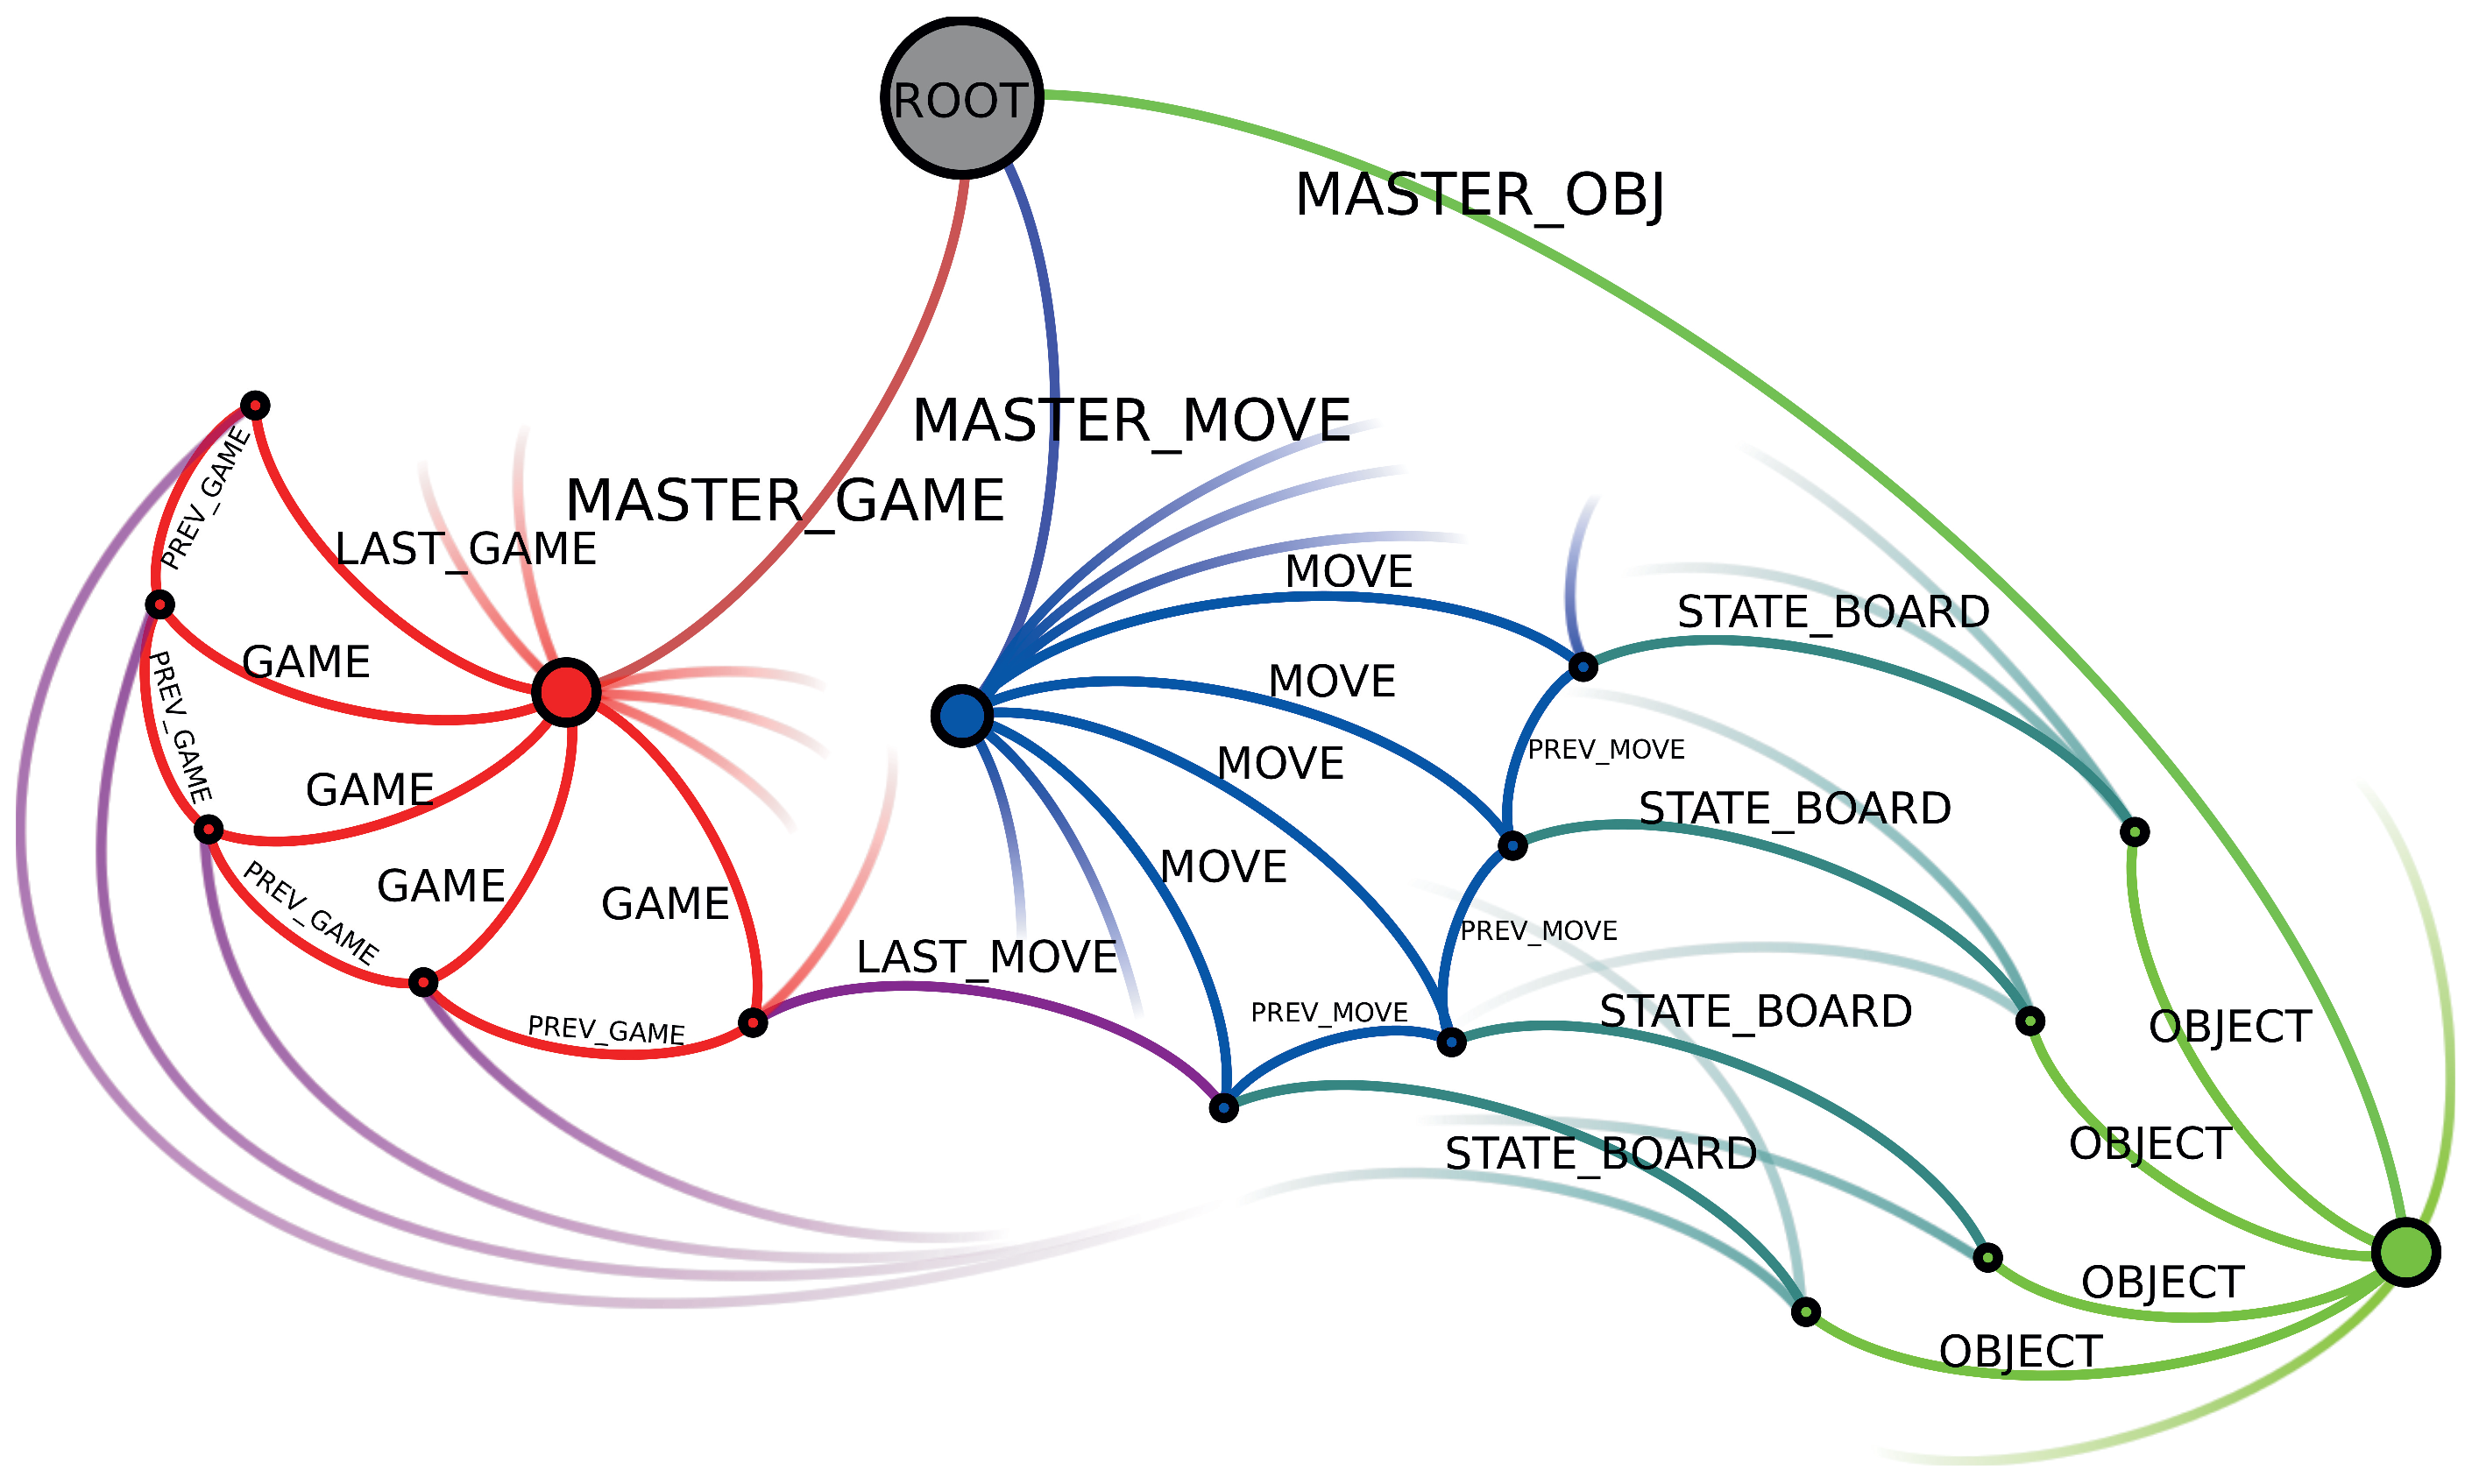
\includegraphics[width=\textwidth]{files/neo4j/episodic_graph}
\caption{Représentation de la mémoire épisodique dans Neo4j.}
\label{episodic_graph}
\end{figure}

\subsection{Vision globale de la mémoire}

La figure~\ref{full_graph} présente le stockage de la mémoire épisodique et de la mémoire sémantique dans Neo4j. Les relations de type \texttt{BOARD\_STATE} assure la liaison entre ces deux mémoires.
\begin{figure}[H]
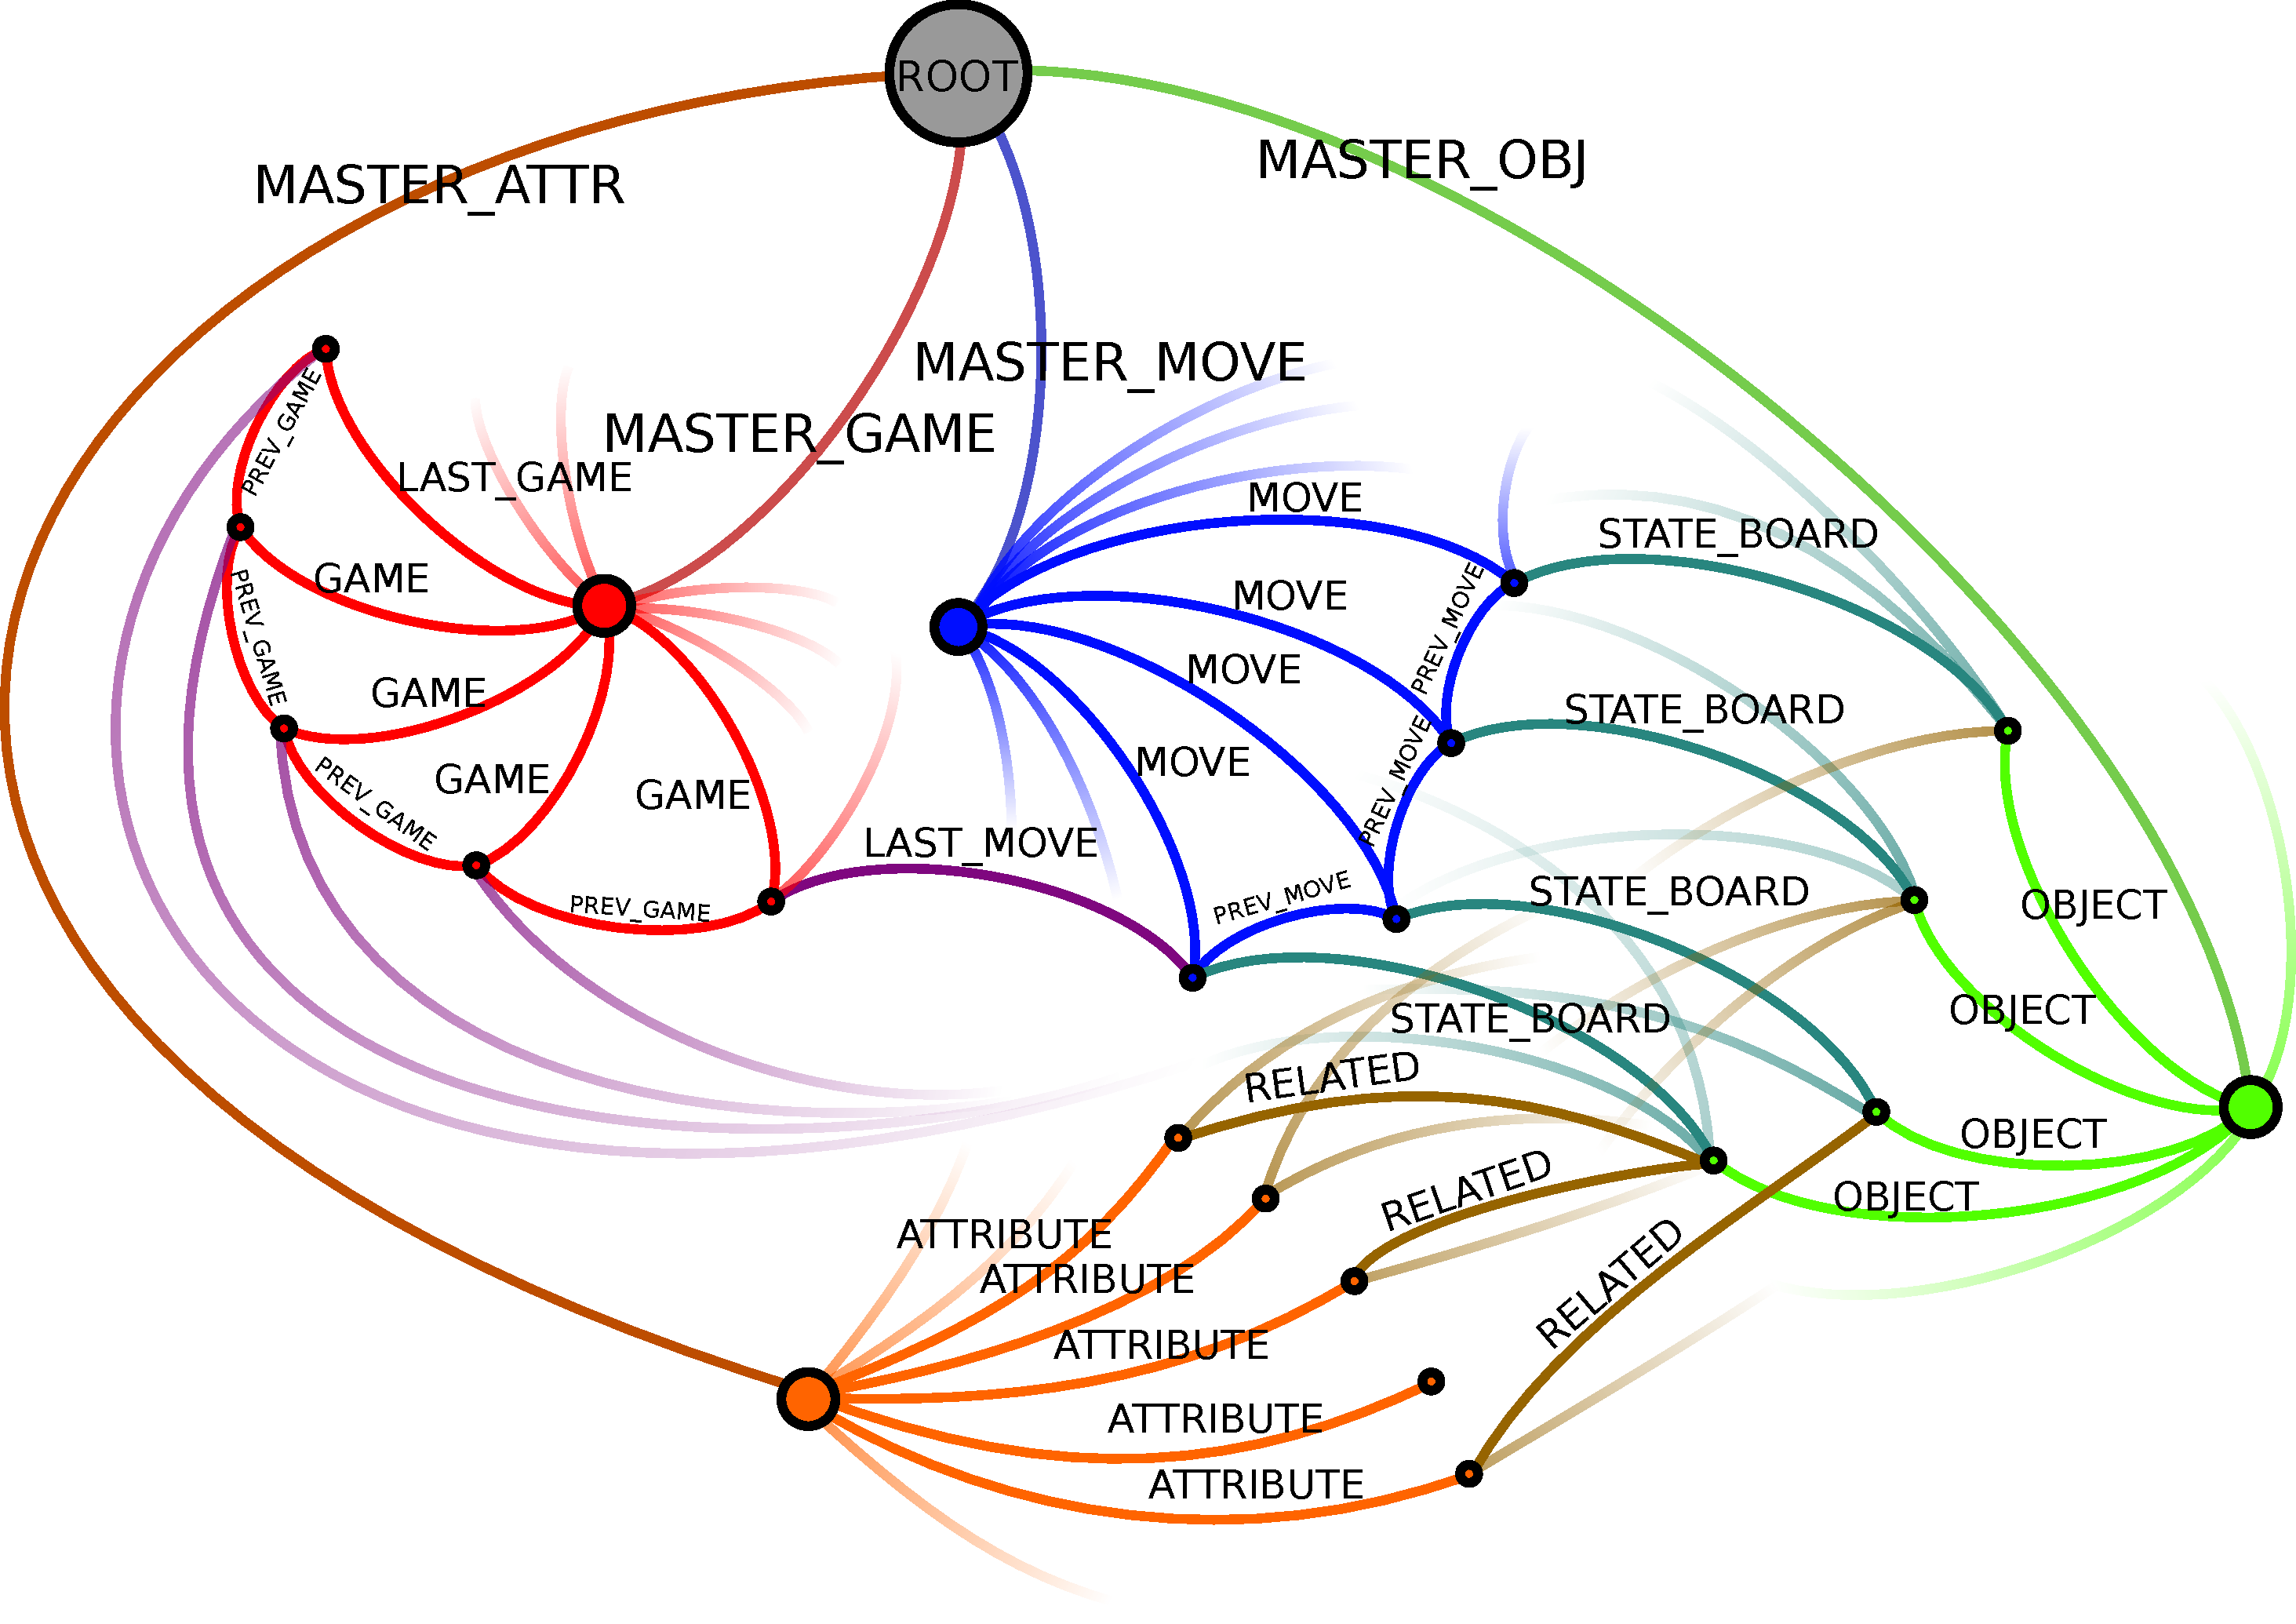
\includegraphics[width=\textwidth]{files/neo4j/full_graph}
\caption{Représentation complète de la mémoire stockée dans Neo4j.}
\label{full_graph}
\end{figure}